\chapter{Concurrency and Threads in .NET}
TODO: Chapter introduction

\section{Concurrency terminology}
This section defines common terminology used in this thesis. These terms are often used in the same context, but even though they are similar, they have different meanings. It is imperative to be aware of these distinctions in order to be able to reason clearly about software and multithreading.

\subsection{Sequential programming}
\emph{Sequential programming} is a way of writing code as a set of step by step instructions. 
It is a convenient, clear approach where mistakes about what to do and when do it are less common.
The disadvantage of performing operations this way is that the thread must wait during parts of the process, being effectively blocked. 
As shown in figure \ref{fig:seq}, sequential programming involves a consecutive, progressively ordered
execution of processes, one instruction at a time in a linear fashion.

\begin{figure}[ht!]
	\centering
		
\includegraphics{figures02/seq.png}
	\caption{Sequential programming involves executing progressively ordered set of instructions}
	\label{fig:seq}
\end{figure}

In imperative and object-oriented languages there is a tendency to write sequential code, with all attention and resources focused on the task currently running. Programs are modeled and executed by performing an ordered set of statements, one after another. \cite{terrell_2018}

\subsection{Concurrent programming}
In computer science, \emph{concurrency} is the ability of different parts of a program, algorithm, or problem to be executed out-of-order or in partial order, without affecting the final outcome. \cite{lamport1978time}
\\ \\ 
Concurrency is used to achieve real multitasking in an application, by modeling the application into multiple, autonomous processes that run at the same in different threads.
As an example let's examine an online video streamer. The program downloads data from the network, decompresses it and displays the video on screen.
Concurrency gives the impression that all of these parts of the program are executing simultaneously, an illusion of parallelism is created. 
But in a single-core environment, the execution of one thread is temporarily paused and switched to another thread, this is called context switching, as shown in \ref{fig:convspar}

\begin{figure}[ht!]
	\centering
		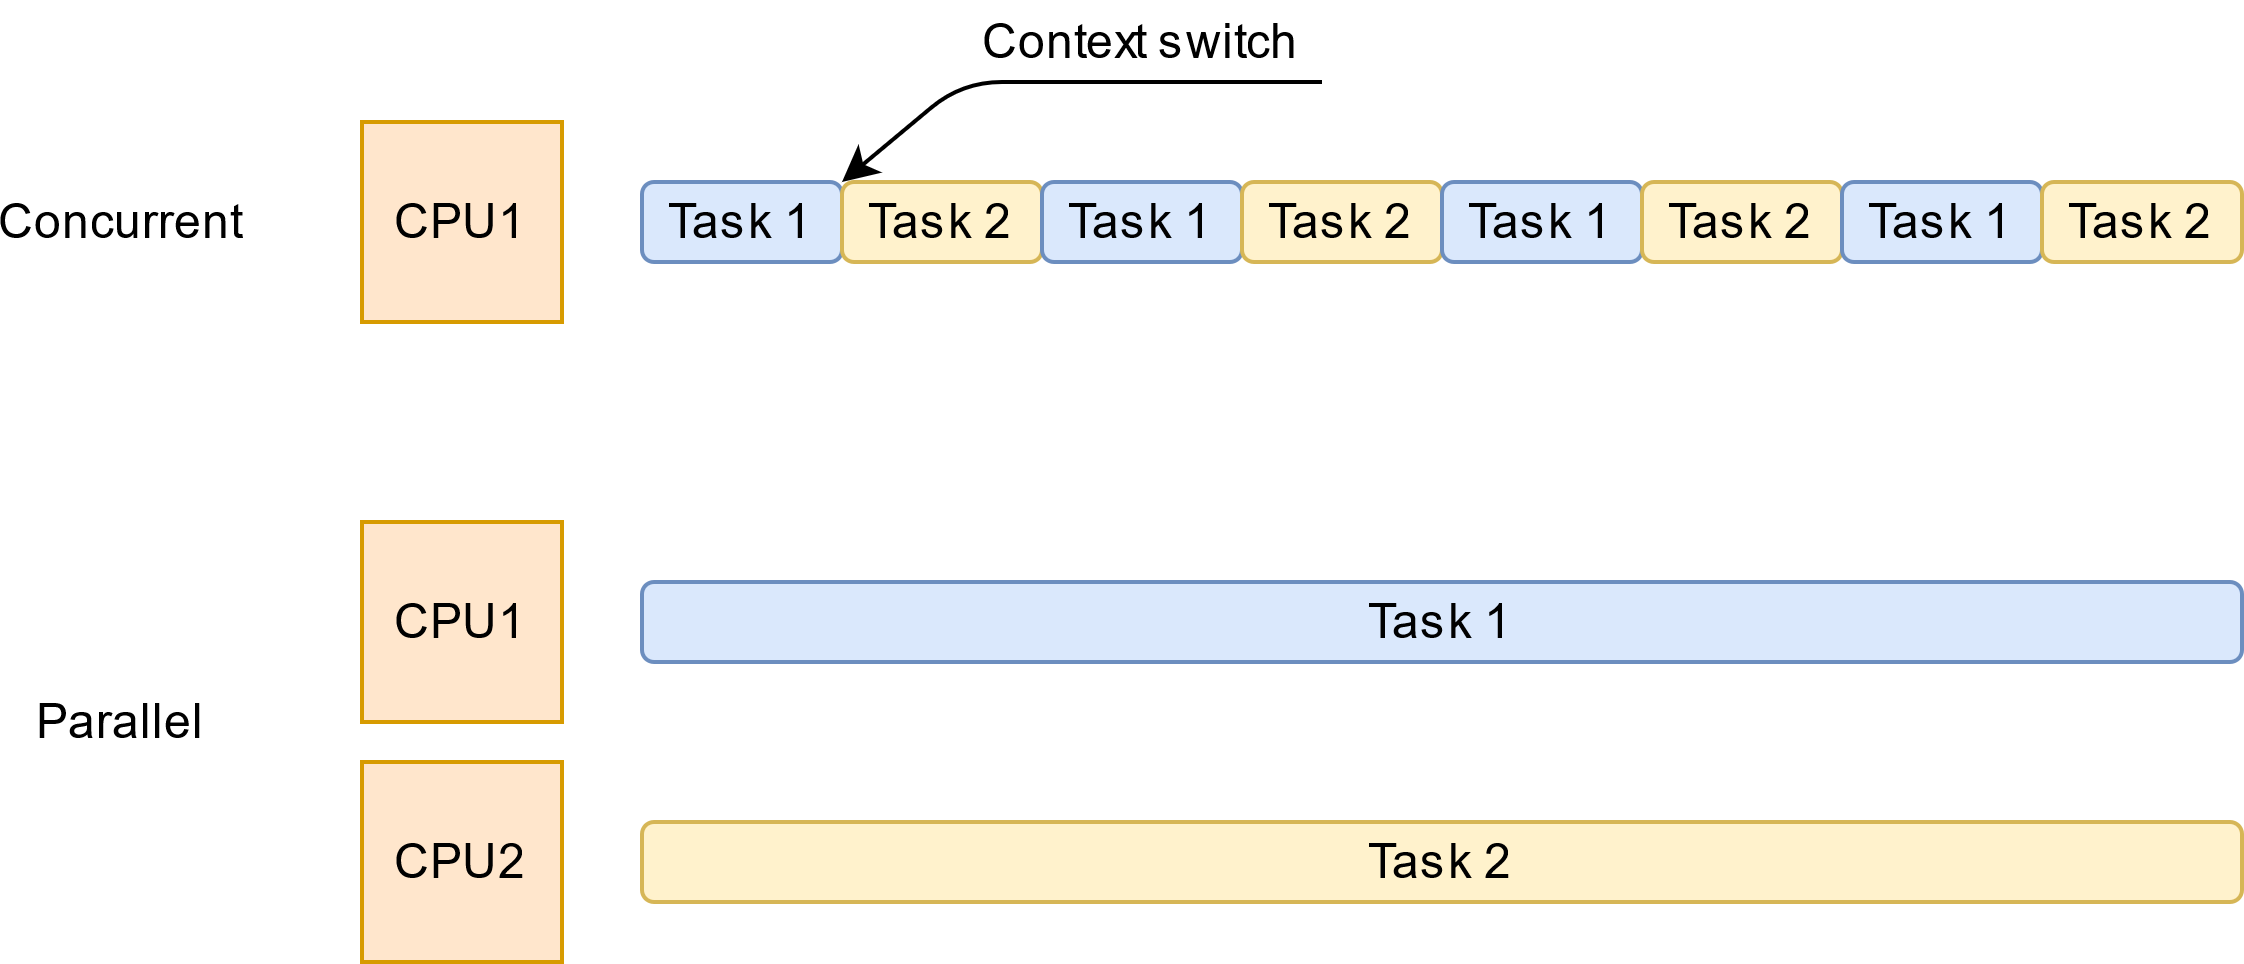
\includegraphics{figures02/convspar.png}
	\caption{Difference between concurrent and parallel models, both may look identical to the user}
	\label{fig:convspar}
\end{figure}

Concurrency is often confused with parallelism \cite{waza}, but concurrent programs only \emph{may} be executed in parallel 
by assigning each process to a separate processor or processor core, or distributing a computation across a network \cite{mordechai}

\subsection{Parallel programming}
Parallelism is the idea of processing tasks simultaneously, literally at the same time on different cores, for perfomance gains puroposes.

Although all parallel programs are concurrent, we have seen that not
all concurrency is parallel. That�s because parallelism depends on the actual runtime
environment, and it requires hardware support (multiple cores). Parallelism is achievable
only in multicore devices (figure 1.4) and is the means to increasing performance
and throughput of a program.
Parallelism can be achieved when a single task is split into multiple independent
subtasks, which are then run using all the available cores. In figure 1.5, a multicore
machine (two coffee stations) allows parallelism for simultaneously executing different
tasks (two busy baristas) without interruption.
The concept of timing is fundamental for simultaneously executing operations in
parallel. In such a program, operations are concurrent if they can be executed in parallel,
and these operations are parallel if the executions overlap in time

\begin{figure}[ht!]
	\centering
		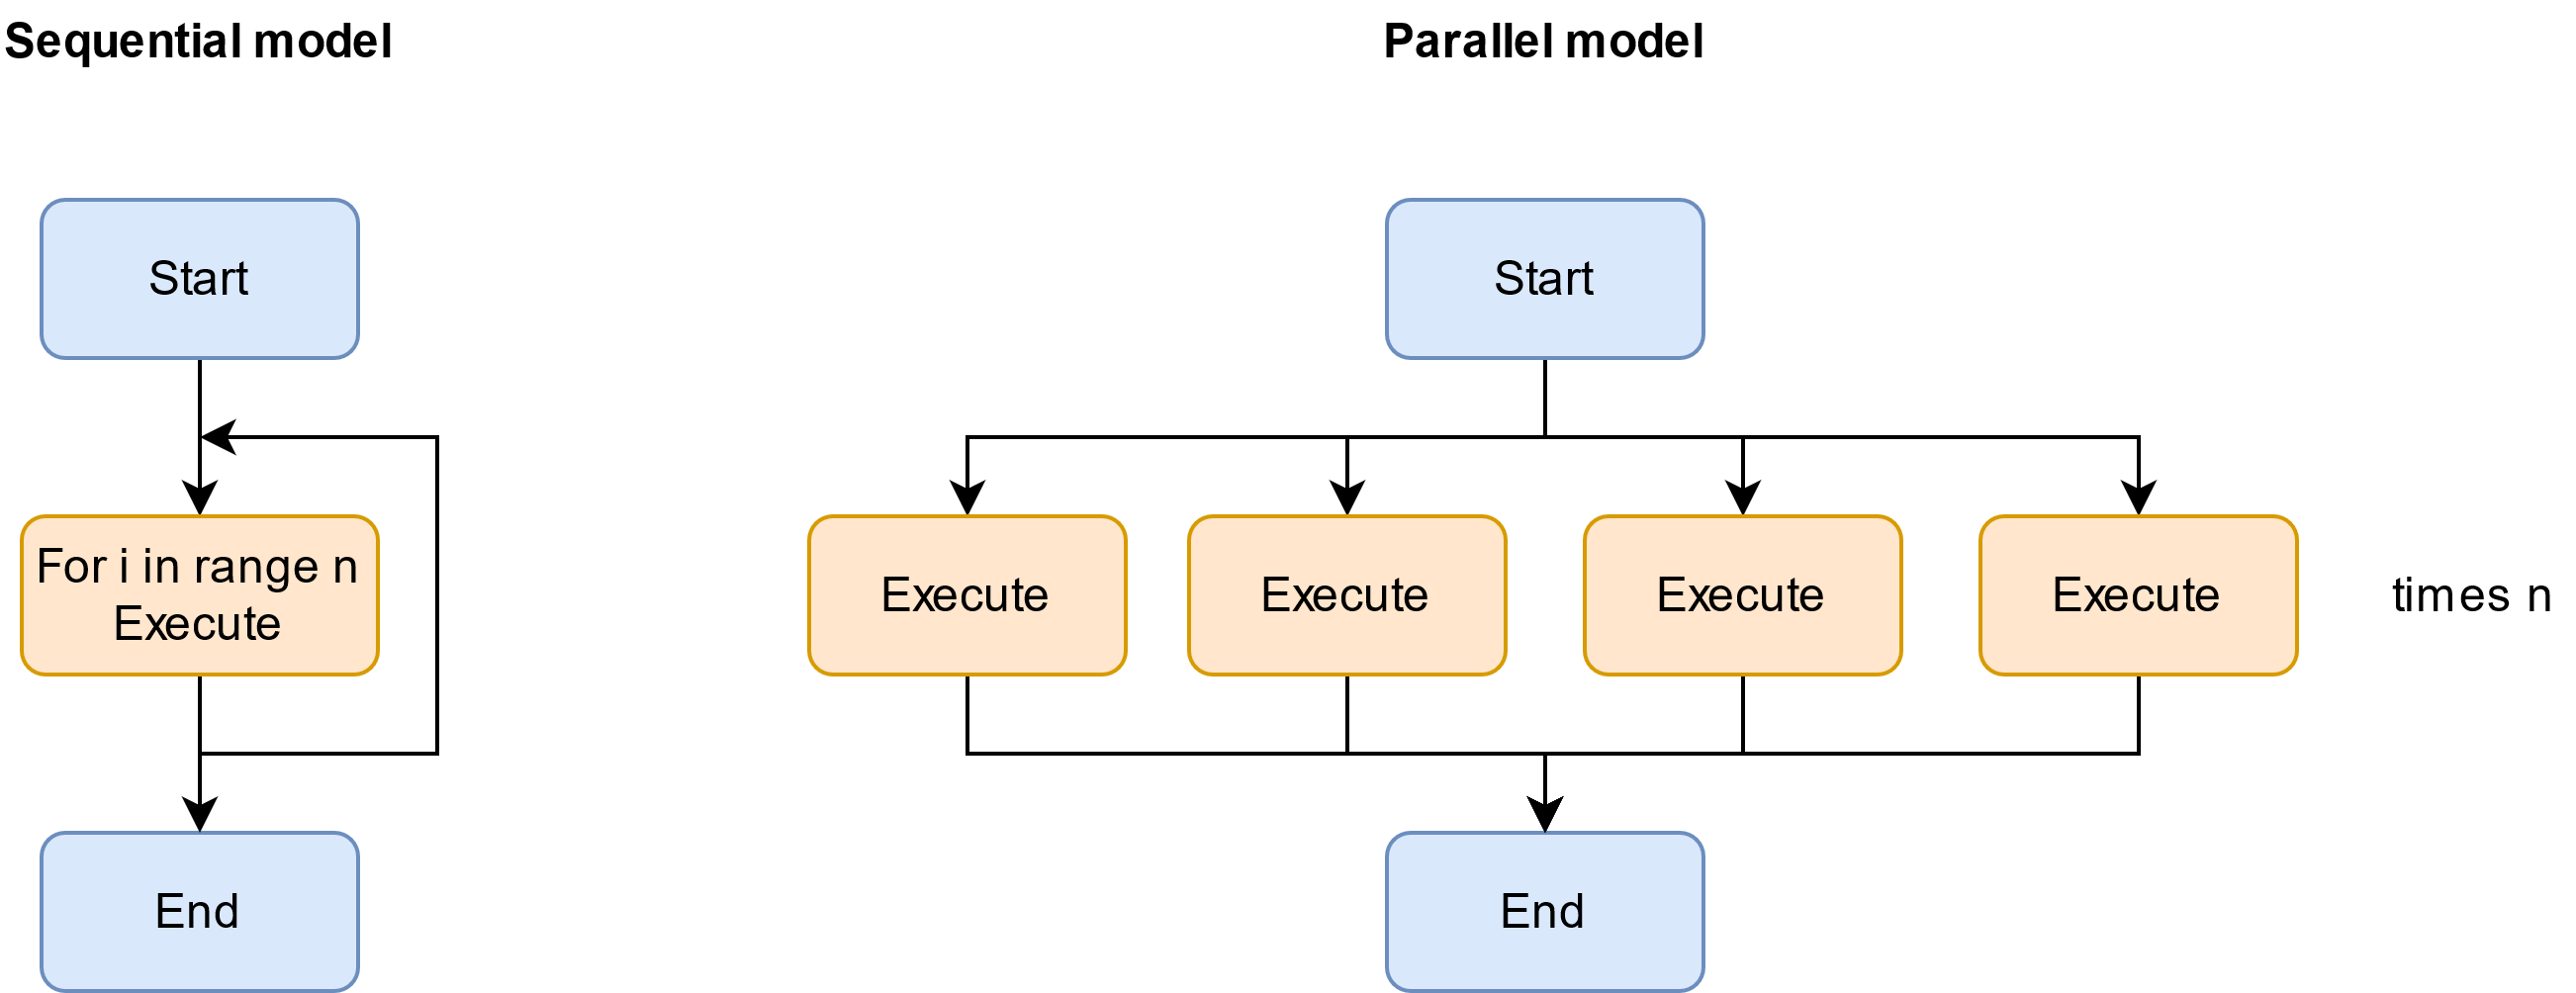
\includegraphics{figures02/seqvspar.png}
		\caption{Comparison of sequential and parallel models}
	\label{fig:seqvspar}
\end{figure}

\subsection{Multitasking}
Multitasking is the concept of performing multiple tasks over a period of time by executing
them concurrently. We�re familiar with this idea because we multitask all the
time in our daily lives. For example, while waiting for the barista to prepare our cappuccino,
we use our smartphone to check our emails or scan a news story. We�re doing
two things at one time: waiting and using a smartphone.
Computer multitasking was designed in the days when computers had a single CPU
to concurrently perform many tasks while sharing the same computing resources. Initially,
only one task could be executed at a time through time slicing of the CPU. (Time
slice refers to a sophisticated scheduling logic that coordinates execution between multiple
threads.) The amount of time the schedule allows a thread to run before scheduling
a different thread is called thread quantum. The CPU is time sliced so that each
thread gets to perform one operation before the execution context is switched to
another thread. Context switching is a procedure handled by the operating system to
Let�s start with terminology 11
multitask for optimized performance (figure 1.7). But in a single-core computer, it�s
possible that multitasking can slow down the performance of a program by introducing
extra overhead for context switching between threads.
Context switching on
a single-core machine
Figure 1.7 Each task has a different shade, indicating that the context switch in a single-core machine
gives the illusion that multiple tasks run in parallel, but only one task is processed at a time.
There are two kinds of multitasking operating systems:
? Cooperative multitasking systems, where the scheduler lets each task run until it finishes
or explicitly yields execution control back to the scheduler
? Preemptive multitasking systems (such as Microsoft Windows), where the scheduler
prioritizes the execution of tasks, and the underlying system, considering the priority
of the tasks, switches the execution sequence once the time allocation is
completed by yielding control to other tasks
Most operating systems designed in the last decade have provided preemptive multitasking.
Multitasking is useful for UI responsiveness to help avoid freezing the UI
during long operations.
\subsection{Multithreading}
Multithreading is an extension of the concept of multitasking, aiming to improve
the performance of a program by maximizing and optimizing computer resources.
Multithreading is a form of concurrency that uses multiple threads of execution.
Multithreading implies concurrency, but concurrency doesn�t necessarily imply multithreading.
Multithreading enables an application to explicitly subdivide specific tasks
into individual threads that run in parallel within the same process.
NOTE A process is an instance of a program running within a computer system.
Each process has one or more threads of execution, and no thread can exist
outside a process.
A thread is a unit of computation (an independent set of programming instructions
designed to achieve a particular result), which the operating system scheduler independently
executes and manages. Multithreading differs from multitasking: unlike
multitasking, with multithreading the threads share resources. But this �sharing
resources� design presents more programming challenges than multitasking does. We
discuss the problem of sharing variables between threads later in this chapter in section
1.4.1.
12 chapter 1 Functional concurrency foundations
The concepts of parallel and multithreading programming are closely related. But
in contrast to parallelism, multithreading is hardware-agnostic, which means that it can
be performed regardless of the number of cores. Parallel programming is a superset
of multithreading. You could use multithreading to parallelize a program by sharing
resources in the same process, for example, but you could also parallelize a program by
executing the computation in multiple processes or even
\section{Concurrency in .NET}